\documentclass[11pt]{beamer}
\usetheme{Montpellier}
\usefonttheme[onlymath]{serif}
\usecolortheme{rose}

\usepackage{tikz} \usepackage{graphicx} \usepackage{algorithm} \usepackage[noend]{algpseudocode} \usepackage{caption}
\usepackage{amsmath} \usepackage{pgfplots} \usepackage{float} \usepackage{xcolor} \usepackage{bm}

\setbeamertemplate{navigation symbols}{}
\setbeamerfont{page number in head/foot}{size=\fontsize{9}{11}}
\setbeamertemplate{footline}[frame number]
\setbeamertemplate{section in toc}{\inserttocsectionnumber.~\inserttocsection}
%\setbeameroption{show notes}  % Comment this out to not show the notes.
%\setbeameroption{show only notes}  % Uncomment this to only show notes.

\author{Glenn Galvizo, under Dr. Floyd Reed}
\title{Efficient Parameter Estimation for Human Microsatellite Mutation}
\institute{University of Hawaii at Manoa}

% Has to be in the preamble...
\usetikzlibrary{shapes.geometric, arrows}
\usetikzlibrary{calligraphy}
\usetikzlibrary{pgfplots.groupplots}
\usepgfplotslibrary{external}
\tikzexternalize

\begin{document}
    \begin{frame}[noframenumbering,plain]
        \titlepage
    \end{frame}

	\section{Introduction}\label{sec:i}
	\begin{frame}[noframenumbering,plain]
		\frametitle{Overview}
        \tableofcontents

        \note{
            \footnotesize
            \begin{enumerate}
                \item Introduce research, talk about human history.
                \item Talk about microsatellites, what they are and my mutation model.
                \item How to find the best parameters for my model.
                \item What the best parameters are.
            \end{enumerate}
        }
	\end{frame}

	\begin{frame}
		\frametitle{Brief overview of modern human history:}
        \centering{\includegraphics[scale=0.89]{include/images/modern-human-history.png}}
        \begin{columns}
            \begin{column}{0.6\textwidth}
            \end{column}
            \begin{column}{0.4\textwidth}
                {\tiny
                    \emph{*Image from Campbell \& Tishkoff~\cite{campbellEvolutionHumanGenetic2010}.}
                }
            \end{column}
        \end{columns}

        \note{
            \footnotesize
            \begin{enumerate}
                \item Start with the origin of modern humans.
                \item What do we know about human history?
                \item Graph, x axis is geographical location, y axis is time.
                \item We have some common ancestor in Africa.
                \item Modern humans emerged 200,000 years ago.
                \item We migrated out of Africa 80,000 years ago to Europe and Middle East, then
                    to the rest of the world about 30,000 years after that.
                \item How do we know this?- Variations in DNA!
                \item Basis of research: Explore different evolutionary models using highly variable genetic marker.
            \end{enumerate}
            % Note: Lines in diagram are migration between generations.
        }
	\end{frame}

	\subsection{Problem Statement}\label{subsec:ps}
	\begin{frame}
		\frametitle{What is the goal of this research?}
        \begin{block}{Research Question}
            \emph{Which microsatellite mutation model parameters are the most likely to produce our observed data?}
        \end{block} \medskip

        \begin{block}{Essential Questions}
            \begin{enumerate}
                \item What is a microsatellite?
                \item What is the observed data?
                \item How do microsatellites mutate?
                    What is the model?
                \item How do we simulate evolution?
                \item How can we find the best parameters?
            \end{enumerate}
        \end{block}

        \note{
            \footnotesize
            \begin{enumerate}
                \item Verbatim, my research question is: \ldots
                \item Dissecting this, we get the following essential questions: \ldots
            \end{enumerate}
        }
	\end{frame}

	\section{Microsatellites}\label{sec:mi}
	\subsection{DNA Variation: Tandem Repeats}\label{subsec:dvtr}
    \begin{frame}
        \frametitle{What is a microsatellite?}
        \begin{definition}[Microsatellite]
            A \emph{microsatellite} is a short sequence in DNA, repeated in tandem.
        \end{definition} \bigskip

        \begin{columns}
            \begin{column}{0.4\textwidth}
                \begin{itemize}
                    \item Interested in number of repeats.
                    \item Represent variation in humans.
                    \item Infer human history by tracking changes.
%                    \item More variable than SNP marker~\cite{gemayelJunkVariableTandemRepeats2012}.
                \end{itemize}
            \end{column}
            \begin{column}{0.6\textwidth}
                \begin{equation*}
                    \begin{aligned}
                         \ldots &\text{AACG}\textbf{ATATATATATAT}\text{GGCTA} \ldots \\
                         \ldots &\text{AACG}\textbf{ATATATATAT}\text{GGCTA} \ldots \\
                         \ldots &\text{AACG}\textbf{ATATATAT}\text{GGCTA} \ldots \\
                         \ldots &\text{AACG}\textbf{ATATAT}\text{GGCTA} \ldots \\
                         \ldots &\text{AACG}\textbf{ATAT}\text{GGCTA} \ldots
                    \end{aligned}
                \end{equation*}
            \end{column}
        \end{columns}

        \note{
            \footnotesize
            \begin{enumerate}
                \item Let's start with the first essential question: \ldots
                \item Form of genetic variation in which short sequences of DNA are repeated in tandem.
                \item Variation = how many times this short sequence is repeated.
                \item On the right, five microsatellite variants with AT as the repeated sequence.
                \item One individual in a population can have the variant on top, with 5 repeats of AT.
                    Another individual can have the variant on the bottom, with 2 repeats of AT.
                \item Infer human history by tracking the changes in repeat length over generations.
%                \item A more popular marker for genetic variation is the SNP, but we use microsatellites because they
%                    mutate more often.
%                    More mutations means that we can potentially infer more in a shorter time period.
            \end{enumerate}
        }
    \end{frame}

    \subsection{Microsatellite Data}\label{subsec:md}
    \begin{frame}
        \frametitle{What data are we working with?} \bigskip
        \begin{columns}
            \begin{column}{0.5\textwidth}
                \begin{itemize}
                    \item Working with Columbian GATA samples. \bigskip
                    \item Samples collected from ALFRED (ALlele FREquency Database). \bigskip
                    \item Interested in frequency of repeat length.
                \end{itemize}
            \end{column}
            \begin{column}{0.5\textwidth}
                \centering{\pgfplotsset{compat=1.5}
\pgfmathdeclarefunction{gauss}{2}{%
  \pgfmathparse{1/(#2*sqrt(2*pi))*exp(-((x-#1)^2)/(2*#2^2))}%
}

%\begin{tikzpicture}
%    \begin{groupplot}[
%        group style={
%        group name=my plots,
%        group size=3 by 3,
%        vertical sep=0pt,
%        horizontal sep=2pt,
%        ylabels at=edge left,
%        xlabels at=edge bottom,
%    },
%    ticks=none, xmin=0, xmax=10,
%    domain=0:10, samples=25,
%    width=0.44\linewidth, height=3cm]
%        \nextgroupplot
%        \addplot [very thick,blue!50!black] {gauss(4,1)};
%        \nextgroupplot
%        \addplot [very thick,blue!50!black] {gauss(3,7)};
%        \nextgroupplot
%        \addplot [very thick,blue!50!black] {gauss(7,2)};
%        \nextgroupplot[ylabel=Frequency]
%        \addplot [very thick,blue!50!black] {gauss(2,0.5)};
%        \nextgroupplot
%        \addplot [very thick,blue!50!black] {gauss(5,1)};
%        \nextgroupplot
%        \addplot [very thick,blue!50!black] {gauss(3,0.3)};
%        \nextgroupplot
%        \addplot [very thick,blue!50!black] {gauss(1,1)};
%        \nextgroupplot[xlabel=Repeat Unit]
%        \addplot [very thick,blue!50!black] {gauss(2,2.5)};
%        \nextgroupplot
%        \addplot [very thick,blue!50!black] {gauss(8,8)};
%    \end{groupplot}
%\end{tikzpicture}

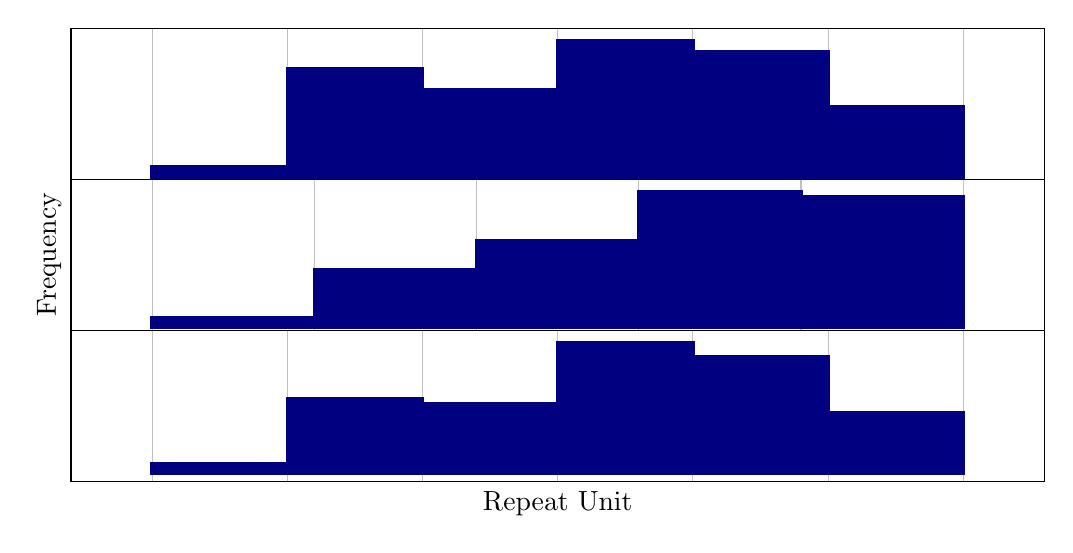
\begin{tikzpicture}
    \begin{groupplot}[
        group style={
        group name=my plots,
        group size=1 by 3,
        vertical sep=0pt,
        horizontal sep=2pt,
        ylabels at=edge left,
        xlabels at=edge bottom,
    },ticks=none, width=1.15\linewidth, height=3.5cm, ybar interval]
        \nextgroupplot
        \addplot+[very thick,blue!50!black] coordinates {
        (8, 0.02) (9, 0.2) (10, 0.16) (11, 0.25) (12, 0.23) (13, 0.13) (14, 0.02)
        };
        \nextgroupplot[ylabel=Frequency]
        \addplot+[very thick,blue!50!black] coordinates {
        (8, 0.02) (9, 0.12) (10, 0.18) (11, 0.28) (12, 0.27) (13, 0.14)
        };
        \nextgroupplot[xlabel=Repeat Unit]
        \addplot+[very thick,blue!50!black] coordinates {
        (8, 0.02) (9, 0.16) (10, 0.15) (11, 0.28) (12, 0.25) (13, 0.13) (14, 0.01)
        };
    \end{groupplot}
\end{tikzpicture}}
            \end{column}
        \end{columns}
%        \bigskip
%        \newline
%        \centering{\emph{Samples of Columbian \text{GATA} microsatellite variations, interested in frequency of a
%        repeat length.}}

        \note{
            \footnotesize
            \begin{enumerate}
                \item Next essential question, \ldots
                \item We are working with observed samples of microsatellites variants.
                \item More specifically, GATA repeat samples from the Columbian population.
                \item Interested in frequency of repeat length in each samples.
                \item We know what a microsatellite is and what data we are working with, how do we get samples?
            \end{enumerate}
        }
    \end{frame}

    \subsection{Mutation Model}\label{subsec:mm}
    \begin{frame}
        \frametitle{How do microsatellites mutate?} \medskip
        \begin{columns}
            \begin{column}{0.55\textwidth}
                \begin{itemize}
                    \item \emph{Single Step}: Mutate up one, down one, or not at all
                        ~\cite{ohtaModelMutationAppropriate2007}. \medskip
                    \item \emph{Proportional:} Mutation rate dependent on
                        length~\cite{ellegrenHeterogeneousMutationProcesses2000} \medskip
                    \item \emph{Focal Bias}: Mutate toward some length~\cite{garzaMicrosatelliteAlleleFrequencies1995}.
                        \medskip
                    \item $\mu_u = $ upward mutation rate \newline
                        $\mu_d = $ downward mutation rate.
                \end{itemize}
            \end{column}
            \begin{column}{0.5\textwidth}
                \centering{\pgfplotsset{compat=1.5}
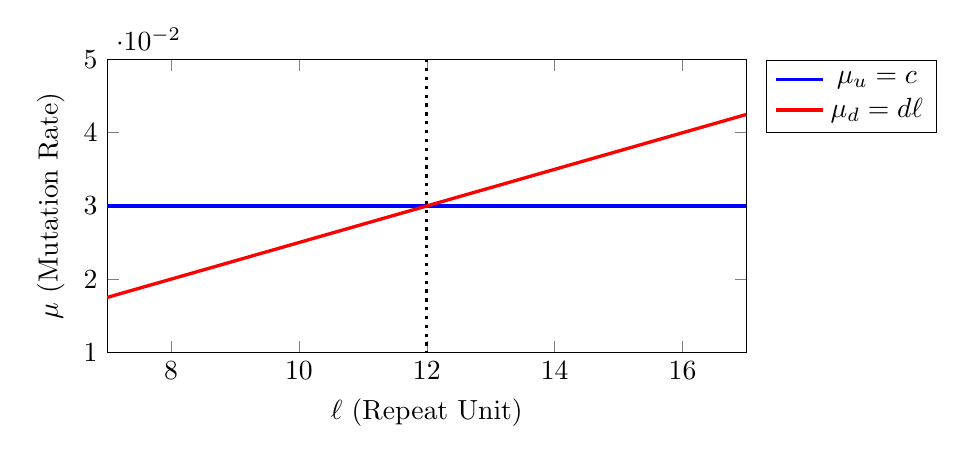
\begin{tikzpicture}
    \begin{axis}[
    width=0.8\linewidth, height=5.3cm,
    ylabel={$\mu$ (Mutation Rate)}, ymin=0.01, ymax=0.05,
    xlabel={$\ell$ (Repeat Unit)}, xmin=7, xmax=17,
    xtick={0, 2, 4, 6, 8, 10, 12, 14, 16, 18, 20, 22, 24, 26},
    samples=100, no markers, legend pos=outer north east, enlargelimits=false,
    domain=0:25
    ]
        \addplot+[very thick]{0.03};
        \addlegendentry{$\mu_u = c$};

        \addplot+[very thick]{0.0025*x};
        \addlegendentry{$\mu_d = d\ell$};

        \addplot+[very thick, black, dotted, forget plot] coordinates {(12, 0) (12, 0.05)};
    \end{axis}
\end{tikzpicture}} \newline
            \end{column}
        \end{columns}

        \note{
            \footnotesize
            \begin{enumerate}
                \item Third essential question: \ldots
                \item We are going to introduce one mutation model with the following points:
                \item Our first point comes from Ohta and Kimura: \ldots
                    Our second point comes from Ellegren: \ldots
                    The third point comes from Garza: \ldots
                \item This brings us to our model: in a graph of mutation rate vs.\ repeat length we have two
                    lines that always intersect each other, using two parameters: $c, d$\ldots
                \item $c$ is the upward mutation rate and $d$ is the linear bias for the downward
                    mutation rate.
                \item This model allows us to move from one generation to the next, how we do simulate lineages and
                    entire populations using this?
            \end{enumerate}
            % Note: We are using a neutral model.
        }
    \end{frame}

    \section{Methodology}\label{sec:m}
	\subsection{Coalescent Simulation}\label{subsec:c}
    \begin{frame}
        \frametitle{How do we simulate evolution?}
        \begin{columns}
            \begin{column}{0.6\textwidth}
                \emph{Answer:} We construct a evolutionary tree (coalescent)! \medskip
                \begin{enumerate}
                    \item Given sample size $n$, mutation parameters $c, d$. \medskip
                    \item Construct random tree with $n$ leaves and common ancestor. \medskip
                    \item Mutate children from an ancestor length until leaves are reached.
                \end{enumerate}
            \end{column}
            \begin{column}{0.4\textwidth}
                \centering{\input{include/floats/present/coalescent-tree.tex}}
            \end{column}
        \end{columns}

        \note{
            \footnotesize
            \begin{enumerate}
                \item Fourth essential question: \ldots
                \item The answer here is to construct an evolutionary tree!
                \item We know how many individuals we have sampled $n$, all we have to do is generate  a random
                    tree that follows the general structure on the right, with $n$ leaves and a common ancestor.
                \item We then randomly define the repeat length of our common ancestor, and mutate down each generation
                    until we reach the bottom.
                    This gives us $n$ repeat lengths, with varying frequencies.
                \item Voila!
                    We have a process to generate data in the same format as our observed data using $c, d$.
                    This leads us to the last question, which $c, d$ are the best?
            \end{enumerate}
        }
    \end{frame}

	\subsection{ABC MCMC}\label{subsec:abcmcmc}
    \begin{frame}
        \frametitle{How can we find the best parameters?}
        \begin{columns}
            \begin{column}{0.6\textwidth}
                \begin{itemize}
                    \item \emph{Problem}: Which model parameters are the most likely to generate our observed data?
                        \begin{enumerate}
                            \item How do we compute this likelihood? \smallskip
                            \item How can we maximize this likelihood?
                        \end{enumerate} \bigskip
                    \item \emph{Solution}: ABC -- MCMC (\footnotesize{Approximate Bayesian Computation -- Markov
                        Chain Monte Carlo})
                \end{itemize}
            \end{column}
            \begin{column}{0.4\textwidth}
                \begin{flushleft}
                    \pgfplotsset{compat=1.5}
\pgfmathdeclarefunction{gauss}{2}{%
  \pgfmathparse{1/(#2*sqrt(2*pi))*exp(-((x-#1)^2)/(2*#2^2))}%
}

\begin{tikzpicture}
    \begin{axis}[
    width=\linewidth, height=6.4cm,
    ylabel={Likelihood}, ymax=0.4,
    xlabel={Parameter Value}, xmin=-5, xmax=10,
    samples=100, no markers, enlargelimits=false, legend style={at={(0.5,-0.35)},anchor=north},
    domain=-25:25, ticks=none
    ]
    \addplot [very thick,blue!50!black] {gauss(4.9,1.5) + gauss(1,2.0)};

    \addplot+[very thick, black, dashed] coordinates {(-5, 0.3) (25, 0.3)};
    \end{axis}
\end{tikzpicture}
                \end{flushleft}
            \end{column}
        \end{columns}

        \note{
            \footnotesize
            \begin{enumerate}
                \item Last essential question: \ldots
                \item More specifically, our question is \ldots
                \item There are two subquestions here: \ldots
                \item The solution I'm presenting today is ABC-MCMC \ldots
            \end{enumerate}
        }
    \end{frame}

    \begin{frame}
        \frametitle{How do we compute likelihood?}
        \begin{columns}
            \begin{column}{0.6\textwidth}
                \begin{itemize}
                    \item \emph{Naive Approach}: Count number of exact matches. \medskip
                    \item \emph{Problem}: Frequency of exact matches is low. \medskip
                    \item \emph{Solution}: Count approximate matches instead!
                        \begin{enumerate}
                            \item Compute distance between generated and observed samples.
                            \item Count number of generated samples where distance is below some threshold.
                            \item Results in wider and flatter
                                distribution (red vs.\ blue)~\cite{lintusaariFundamentalsRecentDevelopments2017}.
                        \end{enumerate}
                \end{itemize}
            \end{column}
            \begin{column}{0.4\textwidth}
                \begin{flushleft}
                    \pgfplotsset{compat=1.5}
\pgfmathdeclarefunction{gauss}{2}{%
  \pgfmathparse{1/(#2*sqrt(2*pi))*exp(-((x-#1)^2)/(2*#2^2))}%
}
\pgfmathdeclarefunction{smallergauss}{2}{%
  \pgfmathparse{0.03/(#2*sqrt(2*pi))*exp(-((x-#1)^2)/(2*#2^2))}%
}

\begin{tikzpicture}
    \begin{axis}[
    width=\linewidth, height=6.4cm,
    ylabel={Likelihood}, ymax=0.03,
    xlabel={Parameter Value}, xmin=0, xmax=40,
    samples=100, no markers, enlargelimits=false, legend style={at={(0.5,-0.35)},anchor=north},
    domain=0:40, ticks=none
    ]
    \addplot [very thick,blue!50!black] {smallergauss(20,1.5)};
    \addplot [very thick,red!50!black] {gauss(20,20)};

    \end{axis}
\end{tikzpicture}
                \end{flushleft}
            \end{column}
        \end{columns}

        \note{
            \footnotesize
            \begin{enumerate}
                \item Our first part: \ldots
                \item How do we find likelihood in general: find the probability of data given a model, repeat for all
                    datum, multiply them together.
                \item We could simulate a population several times, and find out how frequently we generate an exact
                    match to get this probability\ldots
                \item But the frequency of exact matches is small.
                    We have a dimension for each repeat length, all of which can take certain values from 0 to 1.
                \item The solution here, is to count approximate matches!
                \item On graph of likelihood vs.\ parameter, blue line represents our true likelihood -- small but more
                    defined.
                    Red line represents approximate likelihood, flatter but taller distribution.
                \item This method slightly distorts our likelihood, but makes the problem tractable.
            \end{enumerate}
        }
    \end{frame}

    \begin{frame}
        \frametitle{How do we maximize likelihood?}
        \begin{columns}
            \begin{column}{0.6\textwidth}
                \begin{itemize}
                    \item \emph{Problem}: Cannot iterate through all possible likelihoods. \bigskip
                    \item \emph{Solution}: Use MCMC!
                        \begin{itemize}
                            \item Randomly samples from $\propto$ likelihood
                                distribution~\cite{lintusaariFundamentalsRecentDevelopments2017}
                            \item Spends longer time in regions of high likelihood.
                            \item Fit frequency to curve, maximize this curve.
                        \end{itemize}
                \end{itemize}
            \end{column}
            \begin{column}{0.4\textwidth}
                \begin{flushleft}
                    \pgfplotsset{compat=1.5}
\pgfmathdeclarefunction{gauss}{2}{%
  \pgfmathparse{1/(#2*sqrt(2*pi))*exp(-((x-#1)^2)/(2*#2^2))}%
}

\begin{tikzpicture}
    \begin{axis}[
    width=\linewidth, height=6.4cm,
    ylabel={Likelihood}, ymax=0.3,
    xlabel={Parameter Value}, xmin=0, xmax=10,
    samples=100, no markers, enlargelimits=false, legend style={at={(0.5,-0.35)},anchor=north},
    domain=0:25, ticks=none
    ]
    \addplot [very thick,blue!50!black] {gauss(5,1.5)};
    \addplot+[very thick, black, dashed] coordinates {(2.5, 0.06631809) (2.5, 0.16131382) (3.5, 0.16131382)};
    \node[black, below] at (axis cs:2.5,0.065){\small{$\theta^{(1)}$}};
    \node[black, below] at (axis cs:3.5,0.155){\small{$\theta^{(2)}$}};

    \addplot+[very thick, black, dashed] coordinates {(3.5, 0.16131382) (3.5, 0.25158882) (4.5, 0.25158882)};
    \node[black, below] at (axis cs:4.5,0.245){\small{$\theta^{(2)}$}};

    \addplot+[very thick, red, dashed] coordinates {(4.5, 0.25158882) (4.0, 0.25158882) (4.0, 0.21296534)};
    \node[red, below] at (axis cs:4.0,0.210){\small{$\theta^{(3)}$}};

    \end{axis}

\end{tikzpicture}
                \end{flushleft}
            \end{column}
        \end{columns}

        \note{
            \footnotesize
            \begin{enumerate}
                \item The second portion of this problem: \ldots
                \item We can determine the likelihood of a single point, but there are an infinite number of points to
                    explore.
                    We can maximize an equation, but don't have that here.
                    In better words, how can we get an equation?
                \item Our solution to this problem involves a technique known as MCMC.
                \item All MCMC does is randomly walk around our distribution, but waits longer in areas of higher
                    likelihood.
                    In our example here, we move up and up, but may jump back down a small amount.
                \item If we record where we have been, we can generate a histogram of our samples.
                \item This is proportional to our likelihood.
                    From here, we fit a curve to this histogram and maximize the curve.
            \end{enumerate}
        }
    \end{frame}

    \section{Results / Discussion}\label{sec:rad}
    \subsection{Likelihood Distribution}\label{subsec:ld}
    \begin{frame}
        \frametitle{What are our results?}

        \centering{
%            Mutation Rate Equations: $\mu_u = c$, $\mu_d = d\ell$
            \pgfplotsset{compat=1.5}

\begin{tikzpicture}
    \begin{groupplot}[
        group style={
        group name=my plots,
        group size=2 by 1,
        vertical sep=0pt,
        horizontal sep=0.02\linewidth,
        ylabels at=edge left,
        xlabels at=edge bottom,
    },
    try min ticks=3, yticklabels={,,}, ymin=0, ymax=10000,width=0.6\linewidth, height=5cm,
    scaled x ticks=false, log ticks with fixed point, ymode=log, max space between ticks=15pt]
        \nextgroupplot[ylabel=$\propto$ Likelihood,xlabel=$c$,xtick={0, 0.025, 0.05},title={Estimation for $\mu_u = c$}]
        %#
%#        Beta [C]: 3.705530864941286, 2232812.765893399, 0.0009188301175513832, 8049.255118639154
%#        Gaussian [C]: 0.014264520929093853, 0.007024466343237617
%#        Gamma [C]: 3.7398328697465413, 0.000904270021379686, 0.003572396871352965
%#
%beta_p = [3.705530864941286, 2232812.765893399, 0.0009188301175513832, 8049.255118639154]
%norm_p = [0.014264520929093853, 0.007024466343237617]
%gamma_p = [3.7398328697465413, 0.000904270021379686, 0.003572396871352965]
%from scipy.stats import beta, norm, gamma
%from numpy import linspace, average, std
%x = linspace(0.0, 0.045)
%gamma_x = gamma.pdf(x, *gamma_p)
%print('Gamma Mean: {}'.format(gamma.mean(*gamma_p)))
%print('Gamma Var: {}'.format(gamma.var(*gamma_p)))
%
%print('\\addplot [very thick, blue!50!black] coordinates {')
%for i in list(zip(x, gamma_x)):
%    print(f'\t({i[0]}, {i[1]})')
%print('};')

\begin{tikzpicture}
    \begin{axis}[try min ticks=3, ymin=0,width=\linewidth, height=7cm,
        log ticks with fixed point]

        %Gamma Mean: 0.014264437264645212

        \addplot+[very thick,green!50!black,hist=density,hist/bins=20] table[y=c]{c.dat};
        \addplot [very thick, blue!50!black] coordinates {
        (0.0, 0.0)
        (0.0009183673469387755, 1.6548253728417245e-05)
        (0.001836734693877551, 1.2444015955257008)
        (0.0027551020408163266, 6.295905426177485)
        (0.003673469387755102, 14.68413866293454)
        (0.004591836734693877, 24.888512973739783)
        (0.005510204081632653, 35.396523435590396)
        (0.0064285714285714285, 45.045498539524424)
        (0.007346938775510204, 53.08784534301197)
        (0.00826530612244898, 59.14423097026527)
        (0.009183673469387754, 63.1194303161893)
        (0.01010204081632653, 65.11527404476122)
        (0.011020408163265306, 65.35527583160568)
        (0.01193877551020408, 64.12558642338784)
        (0.012857142857142857, 61.732137521238926)
        (0.013775510204081631, 58.471773849129754)
        (0.014693877551020407, 54.61452406768136)
        (0.015612244897959184, 50.394215299184665)
        (0.01653061224489796, 46.00499999683035)
        (0.017448979591836732, 41.60182789955365)
        (0.01836734693877551, 37.30335333628741)
        (0.019285714285714285, 33.19617070805118)
        (0.02020408163265306, 29.339601898766674)
        (0.021122448979591837, 25.77051850134586)
        (0.022040816326530613, 22.5078767450507)
        (0.022959183673469385, 19.556784432851252)
        (0.02387755102040816, 16.912017906339162)
        (0.024795918367346938, 14.560972942483826)
        (0.025714285714285714, 12.486074955532004)
        (0.02663265306122449, 10.66669774320224)
        (0.027551020408163263, 9.08065161132637)
        (0.02846938775510204, 7.705305084688225)
        (0.029387755102040815, 6.518402555698974)
        (0.03030612244897959, 5.498635286856238)
        (0.031224489795918367, 4.626016667271721)
        (0.03214285714285714, 3.882105537305416)
        (0.03306122448979592, 3.2501143872638623)
        (0.03397959183673469, 2.7149326961109694)
        (0.034897959183673465, 2.2630898132904766)
        (0.035816326530612244, 1.8826766878394385)
        (0.03673469387755102, 1.5632414213564163)
        (0.037653061224489796, 1.2956700238633028)
        (0.03857142857142857, 1.0720608159231566)
        (0.03948979591836734, 0.8855985659451424)
        (0.04040816326530612, 0.7304325950594981)
        (0.041326530612244894, 0.6015616431362232)
        (0.04224489795918367, 0.49472719495022466)
        (0.043163265306122446, 0.4063161499904914)
        (0.044081632653061226, 0.3332731266611336)
        (0.045, 0.2730222739873946)
        };
    \end{axis}
\end{tikzpicture};
        \nextgroupplot[xlabel=$d$,xtick={0,0.0025, 0.005},title={Estimation for $\mu_d = d\ell$}]
        %#
%#        Beta [D]: 3.985805060058781, 2132647.440473828, 7.271181113657971e-05, 540.0674440238843
%#        Gaussian [D]: 0.0010817960140329823, 0.0005108622854004084
%#        Gamma [D]: 3.999923637443206, 7.202732935297409e-05, 0.0002524473585100419
%#
%beta_p = [3.985805060058781, 2132647.440473828, 7.271181113657971e-05, 540.0674440238843]
%norm_p = [0.0010817960140329823, 0.0005108622854004084]
%gamma_p = [3.999923637443206, 7.202732935297409e-05, 0.0002524473585100419]
%from scipy.stats import beta, norm, gamma
%from numpy import linspace, average, std
%x = linspace(0.0, 0.0035)
%gamma_x = gamma.pdf(x, *gamma_p)
%print('Gamma Mean: {}'.format(gamma.mean(*gamma_p)))
%print('Gamma Var: {}'.format(gamma.var(*gamma_p)))
%
%print('\\addplot [very thick, blue!50!black] coordinates {')
%for i in list(zip(x, gamma_x)):
%    print(f'\t({i[0]}, {i[1]})')
%print('};')

\begin{tikzpicture}
    \begin{axis}[try min ticks=3, ymin=0, width=\linewidth, height=7cm,
        log ticks with fixed point]

        %Gamma Mean: 0.00108179748586739

        \addplot+[very thick,green!50!black,hist=density,hist/bins=20] table[y=d]{d.dat};
        \addplot [very thick, blue!50!black] coordinates {
        (0.0, 0.0)
        (7.142857142857143e-05, 0.0)
        (0.00014285714285714287, 11.016569847103414)
        (0.0002142857142857143, 67.25543581999192)
        (0.00028571428571428574, 171.7643839357827)
        (0.0003571428571428572, 307.4474694887511)
        (0.0004285714285714286, 453.06389835209484)
        (0.0005, 590.4464993970812)
        (0.0005714285714285715, 706.9602196730798)
        (0.0006428571428571429, 795.5737247729368)
        (0.0007142857142857144, 853.8955043739669)
        (0.0007857142857142857, 882.9049656897374)
        (0.0008571428571428572, 885.7415496851416)
        (0.0009285714285714287, 866.7052193810176)
        (0.001, 830.5082122556938)
        (0.0010714285714285715, 781.7616604806781)
        (0.001142857142857143, 724.6571569145684)
        (0.0012142857142857144, 662.7976286885845)
        (0.0012857142857142859, 599.1350452054344)
        (0.0013571428571428573, 535.9793854570629)
        (0.0014285714285714288, 475.05110068836285)
        (0.0015, 417.55661097328647)
        (0.0015714285714285715, 364.27255896830724)
        (0.001642857142857143, 315.6294512004367)
        (0.0017142857142857144, 271.7890170153878)
        (0.0017857142857142859, 232.7122795190267)
        (0.0018571428571428573, 198.21716276453986)
        (0.0019285714285714288, 168.02564835189514)
        (0.002, 141.80121069179063)
        (0.0020714285714285717, 119.17764095099969)
        (0.002142857142857143, 99.78052255381508)
        (0.0022142857142857146, 83.24262686534092)
        (0.002285714285714286, 69.2144150402605)
        (0.002357142857142857, 57.37070218113926)
        (0.002428571428571429, 47.41439070767772)
        (0.0025, 39.078029055292085)
        (0.0025714285714285717, 32.12381022151955)
        (0.002642857142857143, 26.34249801530885)
        (0.0027142857142857147, 21.551659554881358)
        (0.002785714285714286, 17.593490884545723)
        (0.0028571428571428576, 14.33244753628869)
        (0.002928571428571429, 11.652831752763056)
        (0.003, 9.4564409222776)
        (0.0030714285714285717, 7.660345517455424)
        (0.003142857142857143, 6.194837549226725)
        (0.0032142857142857147, 5.0015705089285944)
        (0.003285714285714286, 4.031897461980751)
        (0.0033571428571428576, 3.245404098034281)
        (0.003428571428571429, 2.6086270770222764)
        (0.0035, 2.093944080589916)
        };
    \end{axis}
\end{tikzpicture};
    \end{groupplot}
\end{tikzpicture}


%            \textbf{Focal length $\bm{\hat{\ell} \approx 13}$, \ Effective population size
%            $\bm{N \approx 10,000}$}
        }
%        \begin{align*}
%            \left( \mu_u = c \right) &\rightarrow \left( \hat{\mu_u} = 0.017 \pm 2.0\text{e-}7 \right) \\
%            \left( \mu_d = d\ell \right) &\rightarrow \left( \hat{\mu_d} = (0.0013 \pm 8.0\text{e-}9) \ell \right)
%        \end{align*}
        \begin{columns}
            \begin{column}{0.6\textwidth}
            \end{column}
            \begin{column}{0.4\textwidth}
                {\scriptsize
                    \emph{*Preliminary results given above.}
                }
            \end{column}
        \end{columns}

        \note{
            \footnotesize
            \begin{enumerate}
                \item To finally answer our research question\ldots
                \item Here, a graph of our frequency, proportional to our likelihood, is plotted on the y axis in
                    log scale.
                    The x axis represents our parameter values.
                \item All of the code was written in Python, optimized by Numba, and ran on the Cray supercomputer here
                    at UH.
                \item The optimal values are \ldots
            \end{enumerate}
        }
    \end{frame}

    \subsection{Future Work}\label{subsec:fw}
    \begin{frame}
        \frametitle{What do we do with this?}
        \begin{block}{Mutation Model:}
            \begin{itemize}
                \item Use more samples from different locations.
                \item Verify and test our parameters against different data.
                \item Run more and longer MCMCs.
            \end{itemize}
        \end{block} \medskip

        \begin{block}{Demographic Models:}
            \begin{itemize}
                \item Estimate time, admixture, population size of Africa split.
                \item Integrate Neanderthal, Denisovan populations.
                \item Answer, ``Who did we come from?''
            \end{itemize}
        \end{block}

        \note{
            \footnotesize
            \begin{enumerate}
                \item Where do we go from here?
                \item For this specific research question, we need to use samples from different locations\ldots
                \item We need to verify and test the accuracy of these parameters.
                \item We need to run longer simulations.
                \item After we are confident in our model, we can explore different demographic models to work
                    toward the big question\ldots
            \end{enumerate}
        }
    \end{frame}

%    \subsection{Interpretation}\label{subsec:i}
%    \begin{frame}
%        \frametitle{What does this mean?}
%
%        \centering{
%            \bigskip
%            {\large
%                \begin{equation*}
%                    \hat{c} = 0.017 \pm 2.0\text{e-}7, \hat{u} = 17 \pm 3.1\text{e-}3,
%                    \hat{d} = 0.0013 \pm 8.0\text{e-}9
%                \end{equation*}
%            }
%            {\footnotesize
%                \begin{align*}
%                    \text{Hyperparameters}: \mathit{I} &= 50000, \mathit{SPP} = 100, \tau = 0.5, f = 100, n = 50, \\
%                    g_d &= N(1.65, 0.1), g_c = N(0.002, 0.0002), \\
%                    g_u &= N(0.01, 0.002), \mathcal{D} = \text{Columbian Populace}
%                \end{align*}
%            }
%        }
%        \begin{enumerate}
%            \item Focal bias $\hat{\ell} \approx 14$ repeat units for Columbian sample.
%            \item 100,000
%        \end{enumerate}
%
%        \note{
%            \footnotesize
%            \begin{enumerate}
%                \item
%            \end{enumerate}
%        }
%    \end{frame}

    \section{Conclusion}\label{sec:c}
    \begin{frame}
        \frametitle{Conclusion}
        \begin{itemize}
            \item Microsatellite = a short sequence in DNA repeated in tandem.\medskip
            \item Microsatellites mutate $\pm 1,0$ repeat lengths, toward focal bias.\medskip
            \item Likely parameters ($c, d$) were found with ABC-MCMC.\medskip
            \item Future work = more samples \& MCMC, different demographics models.
        \end{itemize}

        \note{
            \footnotesize
            \begin{enumerate}
                \item To conclude, a microsatellite\ldots
                \item Microsatellites mutate\ldots
                \item We found the parameters of model by\ldots
                \item Future work includes verifying the parameters we found, and exploring different\ldots
            \end{enumerate}
        }
    \end{frame}

    \begin{frame}
        \frametitle{Acknowledgments}
        \begin{block}{Amazing People:}
            \begin{itemize}
                \item Dr. Floyd Reed \smallskip
                \item Reed Lab \smallskip
                \item Undergraduate Showcase \smallskip
                \item UHM Mathematical Biology Committee \smallskip
                \item The Audience
            \end{itemize}
        \end{block}
    \end{frame}

    \begin{frame}
        \frametitle{References \& Questions :-)}
        \tiny
        \bibliographystyle{plain}
        \bibliography{include/references}
    \end{frame}

    \begin{frame}
        \centering{\huge Extra Slides}
    \end{frame}

    \begin{frame}
        \frametitle{Assessing MCMC Convergence (Trace Plots)}
            \vspace*{0.3cm}
            \centering{
            \begin{tikzpicture}
    \begin{axis}[ymin=0,width=\linewidth, height=3.5cm, ylabel=$c$]

        \addplot+[very thick,green!50!black, mark=none] table[x=p, y=c] {trace1.dat};
        \addplot+[very thick,blue!50!black, mark=none] table[x=p, y=c] {trace2.dat};
        \addplot+[very thick,orange!50!black, mark=none] table[x=p, y=c] {trace3.dat};

    \end{axis}
\end{tikzpicture} \newline
            \vspace*{-1cm}
            \begin{tikzpicture}
    \begin{axis}[ymin=0,width=\linewidth, height=3.5cm, ylabel=$d$, xlabel=Iterations]

        \addplot+[very thick,green!50!black, mark=none] table[x=p, y=d] {trace1.dat};
        \addplot+[very thick,blue!50!black, mark=none] table[x=p, y=d] {trace2.dat};
        \addplot+[very thick,orange!50!black, mark=none] table[x=p, y=d] {trace3.dat};

    \end{axis}
\end{tikzpicture}
        }
    \end{frame}

    % Bringing it all together: estimate effective population size, want to
    % "Mutations are scaled by N, we can use this to estimate to the effective population size"
    % Got 10,000, the number we started with
    % Get the variance fro

%    \begin{frame}[noframenumbering, plain]
%        \centering{\huge{Questions? :-)}}
%    \end{frame}

\end{document}